\documentclass{article}
\usepackage{amsmath}
\usepackage{mathtools}
\usepackage{framed}
\usepackage{tikz}
\usepackage{multicol}

\usepackage[a4paper, total={7in, 10in}]{geometry}

\usepackage{graphicx}
\graphicspath{ {./visualizations/} }

\usepackage{hyperref}
\hypersetup{
    colorlinks = true,
    linkcolor = blue,
    filecolor = magenta,
    urlcolor = cyan,
}

%the comments are from Udacity's project proposal template: https://github.com/udacity/machine-learning/blob/master/projects/capstone/capstone_proposal_template.md

\title{Udacity Machine Learning Nanodegree - Capstone Project}
%(approx. 10-15 pages)
\author{Ruslan Kozhuharov}

\begin{document}
\pagenumbering{gobble}
\maketitle
\tableofcontents
\newpage
\pagenumbering{arabic}

\section{Definition}
%(approx. 1-2 pages)
\subsection{Project Overview}
%In this section, look to provide a high-level overview of the project in layman’s terms. Questions to ask yourself when writing this section:
%Has an overview of the project been provided, such as the problem domain, project origin, and related datasets or input data?
%Has enough background information been given so that an uninformed reader would understand the problem domain and following problem statement?
The Kiva organization is a charitable entity that funds underprivileged people around the world through small loans. Such loans are funded on Kiva’s online platform by one or several donors. The loan amount is then disbursed by Kiva associates to financially excluded individuals. Kiva itself does not collect rent on those loans, but Kiva associates could in order to cover their operating costs. Once a loan is repaid, the individual donors could choose another cause and continue their charitable activity. This helps poor communities by:
\begin{itemize}
  \item Fostering economic activity
  \item Providing access to funds for financially excluded individuals
  \item Encouraging entrepreneurial initiative on the part of the borrower
\end{itemize}
In order to improve their reach, however, Kiva needs a good assessment of the poverty levels in their areas of operation. To do that, Kiva has requested in a \href{https://www.kaggle.com/kiva/data-science-for-good-kiva-crowdfunding}{Kaggle challenge} that a poverty score is created based on other data and that score is combined with a data set for Kiva’s loans from the last 2 years.
\hypertarget{prob_statement}{\subsection{Problem Statement}}
%In this section, you will want to clearly define the problem that you are trying to solve, including the strategy (outline of tasks) you will use to achieve the desired solution. You should also thoroughly discuss what the intended solution will be for this problem. Questions to ask yourself when writing this section:
%Is the problem statement clearly defined? Will the reader understand what you are expecting to solve?
%Have you thoroughly discussed how you will attempt to solve the problem?
%Is an anticipated solution clearly defined? Will the reader understand what results you are looking for?
Based on the definition of the Kiva challenge laid out in the Project Overview, the problems we are going to solve are the following:
\begin{enumerate}
  \item Defining the mathematical expression of ‘poverty’
  \item Selecting the necessary regional data sets
  \item Transforming the data set from step 2 to a form usable for modeling
  \item Building the poverty prediction model
  \item Joining the predicted poverty to all records of the Kiva loans data set
\end{enumerate}
\subsubsection{Defining Poverty}
As mentioned above, ‘poverty’ is a subjective notion that we need to convert to a mathematical measure. In defining that measure we need to take into account the following factors:
\begin{itemize}
  \item The measure should be applicable on country as well as on global level.
  \item The measure should be on a scale between 0 to 1 so that it represents a percentage of poverty. This will allow Kiva to report on poverty-affected areas with regards to the measure’s maximum.
  \item The measure should be scalable if corresponding data from more countries is added.
\end{itemize}
With regards to these points, we will define the poverty score as: 1 - predicted normalized total household income. That is, poverty score of 0.8 corresponds to predicted normalized total household income of 0.2. Thus our prediction will always be on scale from 0 to 1, will be applicable to country and global levels and will be scalable as more country profiles are added (the normalized household income will always be from 0 to 1).
\subsubsection{Selecting Data Sets}
There are two main problems that need to be resolved when selecting data sets useful for the modeling task:
\begin{itemize}
  \item Data with the widest possible coverage (World Bank, UN statistics, CIA World Factbook) is averaged out for each country and does not present a nuanced enough picture of the poverty levels. That is, in countries with high GINI coefficient, the average income levels do not provide a sufficient information about areas with a significant deviation from the average (poverty affected areas).
  \item Local country data is presented in different formats. Every country measures different macroeconomic indicators (and sometimes measures the same indicators in different ways). This makes local data, that could eventually be joined together on global level, unreliable. Example: some countries may consider 'unemployment' as the number of working age individuals with no regular employment contract as unemployed. Other countries may consider 'unemployment' as individuals who do not have a regular employment contract AND are looking for employment (i.e. individuals who are not actively looking for jobs are not counted).
\end{itemize}

To address these issues, we will select the country where Kiva grants the highest number of loans. We will focus exclusively on that country and find a detailed dataset, preferably containing raw data. We will then build an adequate model for the selected country and reduce the number of variables to a few, easily obtainable for other countries. This will make our model, although localized, scalable.

The country receiving the most Kiva loans at this point is the Philippines. Therefore, we will use data from the \href{https://www.kaggle.com/grosvenpaul/family-income-and-expenditure}{Philippines Family Income and Expenditure triennial survey (FIES)}. The data contains information about families’ incomes, expenses, and living conditions (with detailed information about accommodation types, running water, electricity, communications devices, family size, education, etc.). The data set is published on Kaggle and is produced by the Philippines Statistics Authority (PSA).

This data set will be used to derive a model that can predict poverty out of the available features. The poverty score will then be grouped by region and household head gender. We will also derive the administrative regions from the Kiva data set and join the calculated poverty score by region and gender of the borrower.

\subsubsection{Transforming The Data}
Since the data set we will utilize will contain raw data, we will need to transform it to numerical or one hot encoded features. We will perform this work separately in a data transformation phase.
\subsubsection{Building The Poverty Prediction Model}
Once we have transformed the FIES data, we will need to find eventual correlations, remove irrelevant fields and prepare for modeling. We will then proceed and try the effectiveness of several out of the box models (we will refer to them as ‘candidate models’) against three dummy predictors.

The dummy predictors will always predict poverty scores of 0, 0.5 and 1, respectively. We will then compare the performance of the candidate models against the dummy predictors based on the evaluation metrics defined in the next chapter. Finally, we will select the best performing model and improve on it.

The improvement will consist of selecting the features with highest predictive potential and discarding the rest. This will allow Kiva to easily integrate the model in their operation (by simply adding the 3-5 new questions to their loan application form).
\subsubsection{Joining The Predicted Poverty To Existing Kiva Data}
In this phase, we will find an appropriate way to join the results of the poverty prediction model to the existing Kiva loans data set. We will join the poverty scores by borrower gender and region.
\subsection{Metrics}
%In this section, you will need to clearly define the metrics or calculations you will use to measure performance of a model or result in your project. These calculations and metrics should be justified based on the characteristics of the problem and problem domain. Questions to ask yourself when writing this section:
%Are the metrics you’ve chosen to measure the performance of your models clearly discussed and defined?
%Have you provided reasonable justification for the metrics chosen based on the problem and solution?
We will utilize the following evaluation metrics for the household income prediction:
\begin{itemize}
  \item Mean squared error:
    \begin{equation}
      MSE(y, \hat{y}) = \frac{1}{n_{samples}}\sum_{i=0}^{n_{samples} - 1}(y_i - \hat{y}_i)^2
    \end{equation}
  \item R2 score:
    \begin{equation}
      R^2(y, \hat{y}) = 1 - \frac{\sum_{i=0}^{n_{samples} - 1}(y_i - \hat{y}_i)^2}{\sum_{i=0}^{n_{samples} - 1}(y_i - \bar{y}_i)^2}
    \end{equation}
  \item Mean squared logarithmic error:
    \begin{equation}
      MSE(y, \hat{y}) = \frac{1}{n_{samples}}\sum_{i=0}^{n_{samples} - 1}(log_e(1 + y_i) - log_e(1 + \hat{y}_i))^2
    \end{equation}
  \item Explained variance score:
    \begin{equation}
      EV(y, \hat{y}) = 1 - \frac{Var\{y - \hat{y}\}}{Var\{y\}}
    \end{equation}
\end{itemize}
\section{Analysis}
%(approx. 2-4 pages)
\subsection{Data Exploration}
%In this section, you will be expected to analyze the data you are using for the problem. This data can either be in the form of a dataset (or datasets), input data (or input files), or even an environment. The type of data should be thoroughly described and, if possible, have basic statistics and information presented (such as discussion of input features or defining characteristics about the input or environment). Any abnormalities or interesting qualities about the data that may need to be addressed have been identified (such as features that need to be transformed or the possibility of outliers). Questions to ask yourself when writing this section:
%If a dataset is present for this problem, have you thoroughly discussed certain features about the dataset? Has a data sample been provided to the reader?
%If a dataset is present for this problem, are statistics about the dataset calculated and reported? Have any relevant results from this calculation been discussed?
%If a dataset is not present for this problem, has discussion been made about the input space or input data for your problem?
%Are there any abnormalities or characteristics about the input space or dataset that need to be addressed? (categorical variables, missing values, outliers, etc.)
We are using two main data sets: the Kiva loans dataset and the Philippines Family Income and Expenditure Survey (FIES). Both of the datasets are not immediately suitable for the tasks laid out in the \hyperlink{prob_statement}{Problem Statement}. This means that we will have to transform the data in certain ways. We will now look at each data set and its corresponding data transformation.
\subsubsection{Kiva Loans Data Set}
The Kiva loans data set contains 671205 records for loans granted by Kiva in the last 2 years. For the purpose of this project we will use the following columns:
\begin{itemize}
  \item Id: The unique identifier for each loan record. It has a numeric value.
  \item Country: The name of the country where the loan was granted in camel case. We will use this column to select all records from the Philippines.
  \item Region: Unstructured representation of an administrative entity that is below the level of a country. The entity could be a city, city and a province name separated by comma, village name, other geographic entities or no value. We will use this column to derive the actual administrative region in the Philippines where the loan was granted. The derived administrative region will be further used to join the poverty score by region.
  \item Borrower\_gernders: The unique categories in this column are ‘male’ and ‘female’. However, the column’s values could be any combination of those two that is as long as the number of borrowers (e.g. ‘female’, ‘female’, ‘male’ for 3 borrowers of the same loan record). We use this column to derive a borrower gender female one hot encoded column. The new column will be subsequently used to join the poverty score by gender.
\end{itemize}
Here is a sample of the contents of the above-mentioned columns for 5 records:

\begin{center}
\begin{tabular}{ |l|l|l|l| }
  \hline
  id & country & region & borrower\_genders \\
  \hline
  1209550 & Philippines & Dipolog -Zamboanga del Norte & female \\
  888025 & Nicaragua & Masaya & female, female, female \\
  1171969 & Philippines & Roxas Palawan & female \\
  867403 & El Salvador & NaN & male \\
  742400 & Nigeria & Kaduna & female \\
  \hline
\end{tabular}
\end{center}

As we can see from this short example, the ‘region’ column could contain a ‘<city> <province>’ tuple (for loan id 1209550, where the city is Dipolog and the province is Zamboanga del Norte), only city (Masays for loan id 888025), municipality name (Roxas Palawan for loan id 1171969) or no valid value (‘NaN’ for loan id 867403). We will need to transform this column to a standard value using matching tables and other heuristics.

For the records from the Philippines, the unique values for the ‘borrower\_genders’ column are only: ‘female’, ‘male’ and NaN. That’s why will also transform the ‘borrower\_genders’ column by mapping the ‘female’ category to 1 and the ‘male’ category to 0. There are only 80 records with missing values (NaN), so we could do away with them.

\subsubsection{Philippines Family Income and Expenditure Survey}
The Philippines Family Income and Expenditure Survey (FIES) contains 41544 records of household incomes, expenditure, living conditions and other affluence indicators. The data set contains 59 columns representing information in the following categories:

\begin{itemize}
  \item Demographics
    \begin{multicols}{2}
      \begin{itemize}
        \item Agricultural Household indicator
        \item Household Head Sex (categorical)
        \item Household Head Age (categorical)
        \item Household Head Marital Status (categorical)
        \item Type of Household (categorical)
        \item Total Number of Family members
        \item Members with age less than 5 year old
        \item Members with age 5 - 17 years old
        \item Region (categorical)
        \item Household Head Highest Grade Completed (categorical)
      \end{itemize}
    \end{multicols}
  \item Expenses
    \begin{multicols}{2}
      \begin{itemize}
        \item Total Food Expenditure
        \item Bread and Cereals Expenditure
        \item Total Rice Expenditure
        \item Meat Expenditure
        \item Total Fish and marine products Expenditure
        \item Fruit Expenditure
        \item Vegetables Expenditure
        \item Restaurant and hotels Expenditure
        \item Alcoholic Beverages Expenditure
        \item Tobacco Expenditure
        \item Clothing, Footwear and Other Wear Expenditure
        \item Housing and water Expenditure
        \item Medical Care Expenditure
        \item Transportation Expenditure
        \item Communication Expenditure
        \item Education Expenditure
        \item Miscellaneous Goods and Services Expenditure
        \item Special Occasions Expenditure
        \item Crop Farming and Gardening expenses
      \end{itemize}
    \end{multicols}
  \item Income
    \begin{multicols}{2}
      \begin{itemize}
        \item Main Source of Income (categorical)
        \item Total Income from Entrepreneurial Activities
        \item Household Head Job or Business Indicator (categorical)
        \item Household Head Occupation (categorical)
        \item Household Head Class of Worker (categorical)
        \item Total number of family members employed
      \end{itemize}
    \end{multicols}
  \item Living Conditions
    \begin{multicols}{2}
      \begin{itemize}
        \item Imputed House Rental Value
        \item Type of Building/House (categorical)
        \item Type of Roof (categorical)
        \item Type of Walls (categorical)
        \item House Floor Area
        \item House Age
        \item Number of bedrooms
        \item Tenure Status (categorical)
        \item Toilet Facilities (categorical)
        \item Electricity
        \item Main Source of Water Supply (categorical)
        \item Number of Television
        \item Number of CD/VCD/DVD
        \item Number of Component/Stereo set
        \item Number of Refrigerator/Freezer
        \item Number of Washing Machine
        \item Number of Airconditioner
        \item Number of Car, Jeep, Van
        \item Number of Landline/wireless telephones
        \item Number of Cellular phone
        \item Number of Personal Computer
        \item Number of Stove with Oven/Gas Range
        \item Number of Motorized Banca
        \item Number of Motorcycle/Tricycle
      \end{itemize}
    \end{multicols}
\end{itemize}

It is worth noting that the fields Household Head Occupation and Household Head Class of Worker contain only 34008 non-NULL values. We should also apply some category reduction to the fields, one hot encoding as well as query-friendly names to these fields. In addition, all the categorical fields (marked as 'categorical' in the bullet list above) will require additional transformations. Besides the categoricall transformations, all column names need to be changed so that they are query-friendly.

It is obvious that this dataset will require a significant number of preprocessing modifications. We can group those in the following preprocessing operations:

\begin{itemize}
  \item Mapping column string values to query-friendly names
  \item One hot encoding
  \item Columns merging
  \item Reducing / categorizing unique column values
  \item Renaming columns to query-friendly names
\end{itemize}

We will look at all those preprocessing operations in detail in the \hyperlink{data_prep}{Data Preprocessing} chapter.
\subsection{Exploratory Visualization}
%In this section, you will need to provide some form of visualization that summarizes or extracts a relevant characteristic or feature about the data. The visualization should adequately support the data being used. Discuss why this visualization was chosen and how it is relevant. Questions to ask yourself when writing this section:
%Have you visualized a relevant characteristic or feature about the dataset or input data?
%Is the visualization thoroughly analyzed and discussed?
%If a plot is provided, are the axes, title, and datum clearly defined?
Let us start with the most important question - is the Philippines the region with the highest count of Kiva loans. To answer it, we will group and count the loans by country, sort the results by country and display the 5 countries with the highest loan counts:

\begin{figure}[h]
\caption{Number of Loans Per Region}
\centering
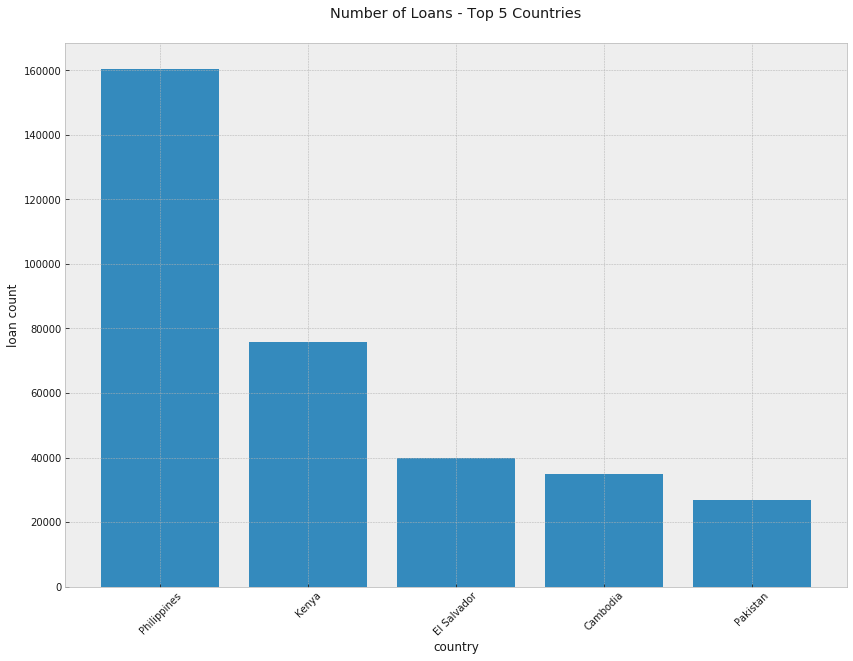
\includegraphics[width = 0.8 \textwidth]{loan_regions}
\end{figure}

As we can see, the Philippines is the region where Kiva mostly focuses their efforts in terms of loan count. Actually, when it comes to loan count, there are twice as many loans granted in the Philippines as in the second country in the list (Kenya).

Now we can focus on the Philippines and the FIES data. We will first derive an estimated family employment feature. It will be defined as: number of employed family members / (total number family members - children). We will also derive ‘no\_electricity’ and ‘no\_running\_water’ indicators.

Let's now plot the estimated family employment by region:

\begin{figure}[h]
\caption{Estimated Employment Per Region}
\centering
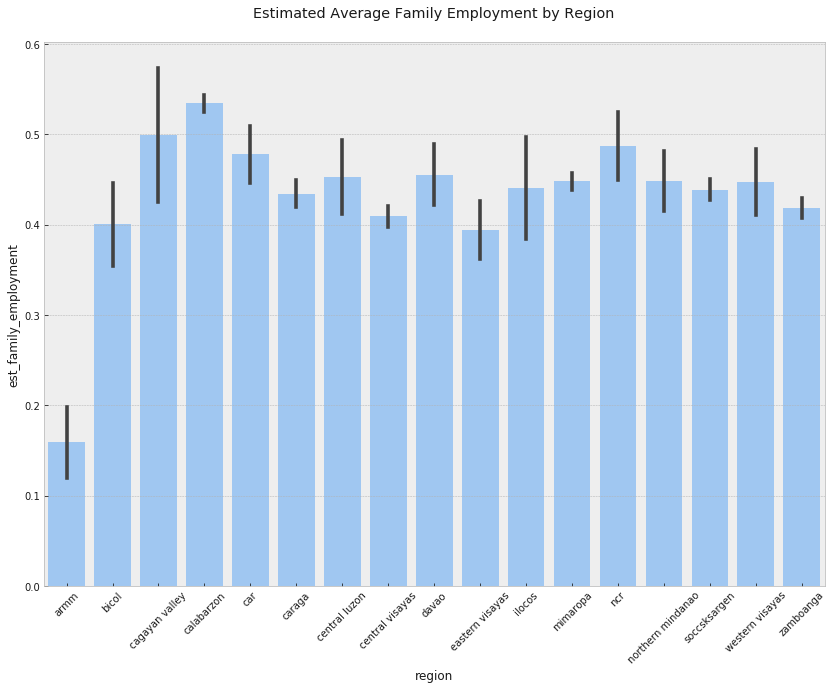
\includegraphics[width = 0.8 \textwidth]{empl_region}
\end{figure}

We can see from the very beginning that the Autonomous Region of Muslim Mindanao (ARMM) is severely affected by unemployment. Another notable feature is that in the Cagayan Valley the disparity in employment between households with male and female heads is greatest.

We continue by visualizing the three major poverty indicators (no running water, no toilet and no electricity):



\section{Methodology}
\hypertarget{data_prep}{\subsection{Data Preprocessing}}

\end{document}
